\chapter{Introduction}\label{sec:intro}

\section{Motivation}\label{sec:intro_motivation}
\begin{marginfigure}[0.8in]
    \centering
	\begin{subfigure}[b]{\textwidth}
    	\centering
        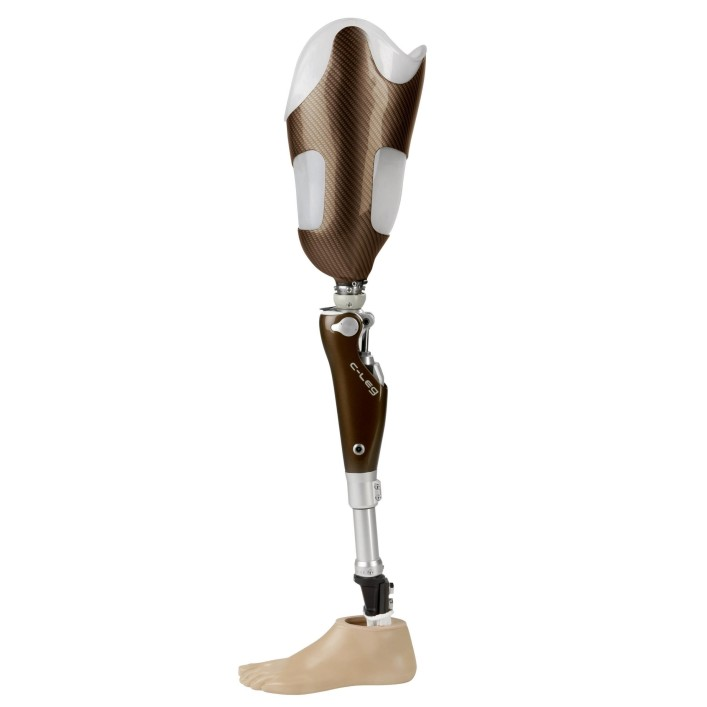
\includegraphics[height=1.5in]{ottobock_cleg}
        \caption{C-Leg™ Knee ©Ottobock}
        \label{fig:ottobock_cleg}
        \vspace{0.25in}
	\end{subfigure}
	\begin{subfigure}[b]{\textwidth}
    	\centering
        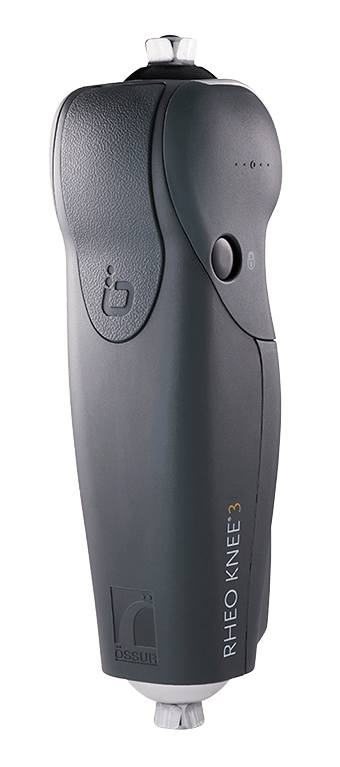
\includegraphics[height=1.5in]{rheo-knee}
        \caption{Rheo™  Knee ©Össur}
        \label{fig:ossur_rheo}
        \vspace{0.25in}
	\end{subfigure}
	\begin{subfigure}[b]{\textwidth}
    	\centering
        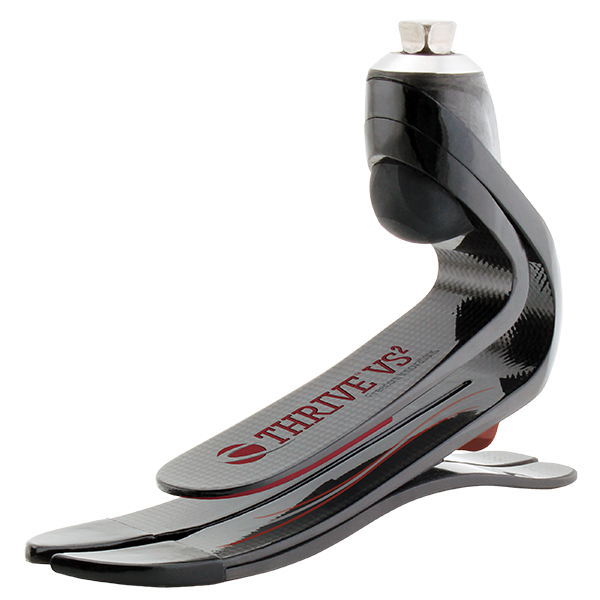
\includegraphics[height=1.5in]{freedom_innov_foot}
        \caption{Thrive™ Foot ©Freedom Innovations}
        \label{fig:freedom_innovations_foot}
	\end{subfigure}
    \caption{Examples of microprocessor-controlled mechanically-passive knee
    prostheses (a,b) and a energy storage and return ankle-foot prosthesis (c).}
\end{marginfigure}
\newthought{Six hundred thousand} lower-limb amputees currently live in the
United States according to recent estimates \citep{ziegler2008estimating}.
People undergo amputations due to a variety of reasons including traumatic
injuries from workplace accidents, traffic collisions, and as casualties of war.
In addition, a large percentage (54\%) suffer from the loss of a limb due to
complications arising from dysvascular disease associated with diabetes.
Consequently, largely due to the expected increase in diabetes in the coming
years, \citet{ziegler2008estimating} estimate that by 2050 the number of
amputees living in the United States will likely double.

Currently, prosthetists often prescribe transfemoral amputees (those with
amputations between the hip and knee joints) an energy storage and return
composite foot such as the Sierra Foot (Freedom Innovations; Irvine, CA;
\cref{fig:freedom_innovations_foot}) along with a microprocessor-controlled,
mechanically-passive knee prosthesis. These knee prostheses feature control
algorithms that measure kinematic and force data via sensors embedded in the
device and adjust the knee's resistance accordingly.  Examples of
microprocessor-controlled prosthetic knees include the C-Leg (Otto Bock;
Duderstadt, Germany; \cref{fig:ottobock_cleg}), which has an adjustable
hydraulic damping system, and the Rheo Knee (Össur; Reykjavik, Iceland;
\cref{fig:ossur_rheo}), which achieves variable damping via a magnetorheological
fluid. While \citet{johansson2005clinical} show these microprocessor-controlled
knees can improve amputee gait characteristics by decreasing metabolic energy
consumption and peak hip torque and increasing gait smoothness over that
provided by fully-passive knee prosthesis, these prostheses still cannot fully
replicate healthy leg behavior as they are incapable of providing positive power
during the gait cycle. 

Positive power at the knee is evident in a number of locomotion tasks including
level walking \citep{perry1992gait}, walking up stairs
\citep{nadeau2003frontal}, running \citep{buczek1990stance}, and jumping
\citep{hubley1983work}. In addition, active knee flexion and extension muscle
activations have been noted during stumble recovery \citep{eng1994strategies}.
At the ankle joint, passive spring-like prostheses cannot replicate the positive
net work seen in the ankle joint during level ground walking, which is essential
for push-off and forward propulsion \citep{perry1992gait}.

Consequently, lower-limb amputees, and especially transfemoral
amputees\sidenote{those with above the knee amputations} equipped with
mechanically-passive prostheses suffer from a number of issues including
markedly increased energy consumption~\citep{waters1976energy},
abnormal gait kinematics~\citep{jaegers1995prosthetic}, and an increased
likelihood of falling~\citep{miller2001prevalence}. Specifically, large
percentages of transfemoral amputees report they are unable to complete tasks
such as walking outside in inclement weather (47.4\%), walking while carrying a
load (42.7\%), walking up or down stairs without a handrail (38.5\%, 37.9\%),
walking outside on uneven terrain (29.5\%), picking up an object from the ground
(28.1\%) or getting up from the floor after a fall (22.8\%)
\citep{gauthier1999enabling}.

Importantly, these gait pathologies can lead an avoidance of walking
\citep{gauthier1999enabling}. This is especially true in the case of falls.
\citet{miller2001prevalence} find 49.2\% of lower limb amputees feared falling
and that of those afraid of falls 76\% avoided physical activity as a result.
Avoidance of physical activity is eminently concerning as it may lead to reduced
strength, endurance, and balance, feeding a positive feedback loop that causes
further debilitation.
\begin{figure*}[b]
    \centering
	\begin{subfigure}[b]{0.3\textwidth}
    	\centering
        %\includegraphics{}
        \missingfigure{Gen 1}
        \caption{Generation 1}
	\end{subfigure}
	\begin{subfigure}[b]{0.3\textwidth}
    	\centering
        %\includegraphics{}
        \missingfigure{Gen 2}
        \caption{Generation 2}
	\end{subfigure}
	\begin{subfigure}[b]{0.3\textwidth}
    	\centering
        %\includegraphics{}
        \missingfigure{Gen 3}
        \caption{Generation 3}
	\end{subfigure}
    \caption{Vanderbilt University's Robotic Transfemoral
    Prostheses.\vspace{0.1in}}
    \label{fig:vanderbilt_prostheses_intro}
\end{figure*}

To help remedy this situation, in the past decade researchers and companies have
developed robotic powered knee and ankle prostheses for lower-limb amputees.
These prostheses feature actuators at the knee and/or ankle that, if controlled
correctly, could potentially restore the kinetics, kinematics, and reactions
of the healthy human leg. Notable examples include three generations of
transfemoral prostheses developed by Vanderbilt
University~(\cref{fig:vanderbilt_prostheses_intro}) \citep{sup2009preliminary,
lawson2013control, lawson2014robotic} and the Biom powered
ankle~(\cref{fig:biom_ankle}) \citep{herr2012bionic}. These powered prostheses
have helped amputees walk on level ground more naturally and efficiently, as
well as walk up stairs and slopes \citep{sup2011upslope, lawson2013control}, run
\citep{huff2012running, shultz2015running}, perform sit-to-stand
\citep{varol2009powered}, and dance \citep{rouse2015design}. These results
illustrate the benefits of powered prostheses as many of these tasks require
positive joint power and thus would be difficult to perform with
mechanically-passive prostheses.

\begin{marginfigure}[-1in]
    \centering
    %\includegraphics{}
    \missingfigure{Biom Ankle}
    \caption{Biom Robotic Ankle Prosthesis}
    \label{fig:biom_ankle}
\end{marginfigure}


\subsection{Challenges in Transfemoral Prosthesis
Control}\label{sec:intro_challenges} 

It still remains an open research question how best to control these prostheses
to achieve natural and robust gaits. In the most established control method for
powered prostheses, the prosthesis uses simple functions to approximate the
joint torque versus angle relationship, termed the \emph{quasi-stiffness}
observed during walking~\citep{sup2007design, lenzi2014speed}. However, since
the torque functions only approximate steady, level walking, this method
requires further tuning to handle other situations such as walking on
slopes~\citep{sup2011upslope} or rough ground~\citep{thatte2016toward} and
changing foot placement targets~\citep{schepelmann2016evaluation}. 

As mentioned earlier, walking on slopes and rough ground present major hurdles
for transfemoral amputees. Moreover, previously developed prosthesis controls
have not specifically addressed the risk of falling that is so detrimental to
amputee quality of life. Therefore, it is clear that we should formulate a
prosthesis controller with more power to generalize to a larger variety of
environments, which will improve amputee gait robustness. Formulating a robotic
prosthesis controller to accomplish this goal requires we address three main
challenges:

\begin{marginfigure}
    \centering
    %\includegraphics{}
    \missingfigure{passive dynamic walker}
    \caption{A passive dynamic walker walks down hill with no internal
    actuation highlighting the role of natural dynamics in walking.}
    \label{fig:passive_dynamic_walker}
\end{marginfigure}

\begin{challenges}
    \item\label{chal:dynamic} \emph{Human locomotion is a dynamic task}~~During
    stance, the leg acts in a compliant, spring-like manner
    \citep{geyer2006compliant} and significant time is spent in
    statically-unstable contact on the heel or toe, suggesting the importance of
    mechanical stability achieved via foot placement \citep{perry1992gait}.
    During swing, ballistic motion explains much of the leg trajectory
    \citep{mochon1980ballistic}. Indeed, much of the entire gait cycle can be
    explained via passive dynamics as evidenced by passive-dynamic walkers
    (\cref{fig:passive_dynamic_walker}) that can stably walk down slight
    inclines with no onboard power source~\citep{mcgeer1990passive,
    collins2005efficient}.

    Consequently, in order to ensure that amputee gaits are natural and
    efficient, but still robust, it is essential that robotic prosthesis
    controllers not only admit, but leverage the inherent dynamics of walking.
    Therefore, the required control paradigm cannot follow strategies often used
    for humanoid locomotion (for example on Honda's Asimo Robot
    \cref{fig:asimo}) that employ position control in order to track preplanned,
    statically-stable gaits. Rather, the control strategy should interact
    dynamically with the amputee by governing interaction forces instead of
    mandating kinematic objectives.

    \begin{marginfigure}
        \centering
        %\includegraphics{}
        \missingfigure{Rheo Knee}
        \caption{Honda's Asimo Robot uses position control and statically
        stable gaits.}
        \label{fig:asimo}
    \end{marginfigure}

    \item\label{chal:incomplete_state} \emph{We have incomplete state
    information}~~An additional difference between robotic prosthesis control
    and controls often used on humanoid walking robots stems from the lack of
    full state information.  Humanoid walking controllers such as those used in
    the DARPA robotics challenge (DRC), controllers use the full state of the
    robot (\ie the positions and velocities of every joint and the robot's
    center of mass), to plan and track a trajectories, thereby ensuring
    stability of the full system \citep{feng2015optimization,
    kuindersma2014efficiently, englsberger2014trajectory}.

    While these recent approaches used in the DRC are dynamic and therefore
    address challenge 1, for prosthesis control we typically only know the state
    of the prosthesis itself. It is unreasonable to expect that amputees will
    don full body sensing suits in order to provide a complete picture of the
    state of the amputee-prosthesis system. Therefore, prosthesis controllers
    must be decentralized, meaning joint torque commands are computed using only
    a subset of the full state. A side affect of this approach is a loss of
    formal stability guarantees. However, we can still evaluate amputee
    stability empirically.

    \item\label{chal:amputees_unique} \emph{Amputees are unique}~~Finally, we
    should be able to adapt robotic prosthesis controllers to each amputee's
    individual needs. The variation in amputee needs arise from a number of
    factors including, but not limited to, the amputee's height, weight,
    strength, endurance, reason for amputation, time since amputation,
    experience, and personal preferences. Consequently, prostheses and
    controllers should be optimized to suit individual users.
\end{challenges}

\vspace{2ex}
\begin{fullwidth} \emph{This thesis proposes dynamic decentralized control
methods for transfemoral prostheses, along with methods to optimize them for
individual amputees, in order to improve gait robustness and naturalness.}
\end{fullwidth}

\subsection{Approach}\label{sec:intro_approach}

In this thesis, we seek to improve amputee gait robustness and naturalness by
employing an alternative approach to joint control in prostheses that seeks to
mimic the underlying dynamics and control of the human neuromuscular system. In
this approach, instead of replicating recorded torque profiles with
quasi-stiffness functions, we model the dynamical system, consisting of virtual
muscles and local reflex feedback pathways, that generate joint torques during
locomotion.  Crucially, the resulting prosthesis control addresses
\cref{chal:dynamic,chal:incomplete_state}: the control is decentralized, as the
reflex feedback are designed to rely only on the state of other muscles in the
same leg, and dynamic, as the virtual muscles integrate the sensed kinematic
state of the prosthesis in order to generate desired torques, not positions, at
the joints. These torques, along with the reaction forces in the amputee's
socket and on the ground shape the motion of the amputee-prosthesis system.
\begin{marginfigure}
    \centering
    %\includegraphics{}
    \missingfigure{muscle ankle}
    \caption{\citet{eilenberg2010control} simulate virtual muscles in
    order to control an ankle prosthesis.}
    \label{fig:eilenberg_muscle}
\end{marginfigure}

Prior work on neuromuscular models shows that when applied to simulated biped
models they can produce robust gaits with natural appearances. For example,
using a neuromuscular model, an optimized simulated biped model walked on
unseen, uneven terrain with sudden drops and steps up to 14 centimeters
\citep{song2015neural}. In addition, \citet{eilenberg2010control} successfully
applied the neuromuscular control approach to a powered ankle prosthesis
(\cref{fig:eilenberg_muscle}), which mimics the kinematics and kinetics of the
ankle joint in human walking including its adaptation to sloped environments. It
remains unclear, however, whether we can extend the approach to transfemoral
prostheses with both knee and ankle joints.

Therefore, to motivate our specific choice of neuromuscular control for
improving amputee gait stability, in completed work, we construct a simulation
of the amputee-prosthesis system and compare the gait robustness achieved by
neuromuscular control versus the established impedance control method. We find
that neuromuscular control enabled the simulated amputee to walk further over
rougher terrain than the established impedance control method allows.

Next, to test the feasibility of the control approach to control a real system,
we design and build a partial powered transfemoral prosthesis prototype with an
active knee actuator and a passive, spring-loaded ankle. The prosthesis
prototype uses series elastic actuation~\citep{pratt1995series} that allows it
to accurately achieve the torques commanded by the neuromuscular model. Initial
tests with an intact user wearing the prosthesis through an amputee simulator
adaptor show that the proposed neuromuscular control, when applied to the knee
of an active prosthesis, produce reasonable kinematics and joint torques. This
positive result motivates continued development of the prosthesis into a full
active knee and ankle transfemoral prosthesis and implementation of testing of
the full neuromuscular prosthesis control.

To address the \cref{chal:amputees_unique}, we propose to optimize prosthesis
controls for specific subjects. To this end, in completed work, we develop an
algorithm that uses preference feedback from users to optimize control system
parameters. We test the method on problems of increasing relevance: first by
optimizing synthetic reward functions, then optimizing the parameters of
simulated dynamical systems, and finally by optimizing neuromuscular control
parameters for intact users wearing the prosthesis through an amputee emulator
brace. The results suggest the proposed optimization method outperforms baseline
methods for optimizing from user preferences. However, it remains to be seen if
the proposed method improves gait characteristics when applied to the full
neuromuscular controlled prosthesis for an amputee subject. We intend to
investigate this question via additional tests on an amputee subject.

Last, we seek to improve the capability of the transfemoral prosthesis to
respond to trips, which pose a significant and impactful threat to amputee
quality of life. To accomplish this goal, we propose to use imitation learning
techniques \citep{argall2009survey} to learn polices that allow the prosthesis
to appropriately respond to disturbances during swing.  The proposed method to
learn these policies will address challenges 1-3 in that it will be a
decentralized control that only uses information from the prosthesis and be
dynamic and personalized by working with each amputee' innate trip response
reflexes.

Previous work in this area has trained classifiers on data obtained by tripping
healthy human subjects~\citep{lawson2010stumble, shirota2014recovery}. The
authors then evaluate these classifiers via cross validation, in which a subset
of the training data is set aside and used for testing, and report low
error-rates.  However, to date no one has applied a trip classifier to
prosthesis hardware in order to initiate a trip recovery controller. Trivial
application of classifiers trained on healthy human subject data likely will
yield poor results, as the distribution of data at test time generated by a
prosthesis that is controlled by a learned policy will differ from the data used
to train that policy. The training and test time distribution mismatch violates
the i.i.d.\sidenote[][1in]{independent and identically drawn} assumption that
underpins classification performance. To remedy this problem, we intend to
employ the DAGGER training method \citep{ross2011reduction} that aligns the
train and test time distributions through an iterative procedure. We will
collect training and testing data to learn and evaluate the trip recovery
policies using the Push Bot robot (\cref{fig:push_bot}) which can apply tripping
forces to subjects via actuated tethers.
\begin{marginfigure}[-3.5in]
    \centering
    %\includegraphics{}
    \missingfigure{push bot}
    \caption{Push Bot robot for training and evaluating trip recovery policies}
    \label{fig:push_bot}
\end{marginfigure}

\section{Expected Contributions}\label{sec:intro_contributions}

Work presented in this thesis will advance the state-of-the-art for robotic
transfemoral prosthesis control and optimization. There are four main expected 
contributions: 

\begin{marginfigure}
    \centering
    %\includegraphics{}
    \missingfigure{prosthesis}
    \caption{Proposed SEA prosthesis design}
    \label{fig:prosthesis_design}
\end{marginfigure}

\begin{contributions}
    \item\label{contrib:pros_design} \emph{A series elastic prosthesis
    design}~~We present the design of a transfemoral prosthesis featuring series
    elastic actuators (SEAs) capable of accurately producing the torques
    commanded by the neuromuscular model, generating enough torque and speed to
    enable trip recovery experiments, and handling the impact loads expected
    during trip recovery experiments. We have made significant progress towards
    this contribution already by completing the design, manufacturing, assembly,
    and initial testing of the prosthesis' knee joint as well as the design and
    fabrication of its ankle joint.  \Cref{fig:prosthesis_design} shows the
    current stage of the prosthesis prototype with the completed SEA knee and a
    passive spring-loaded ankle well as a CAD render of the expected completed
    prosthesis design.

    \item\label{contrib:pref_opt} \emph{A method for optimizing systems via
    preferences}~~We present a new algorithm for optimizing systems, such as
    prostheses, using user preferences.  The algorithm uses preferences between
    pairs of control parameters to circumvent having to define or learn an
    explicit reward function for each user. Additionally, the algorithm employs
    Bayesian optimization techniques in order to query users for preferences
    that are expected to maximally reduce the uncertainty of the location of the
    optimum parameters.

    \item\label{contrib:neuromuc_eval} \emph{Evaluation of neuromuscular
    transfemoral prosthesis control}~~We will implement the proposed
    neuromuscular prosthesis control on the SEA transfemoral prosthesis,
    optimize its parameters according to the amputee subject's preferences, and
    evaluate the prosthesis' ability to produce a natural and robust gait.  We
    will measure gait characteristics in terms of joint kinematics and kinetics
    and the amputee's metabolic energy consumption. We will present results
    relative to typical non-amputee gait, the amputee's gait using his or her
    prescribed prosthesis, and the gait achieved by an unoptimized prosthesis
    control. We will also evaluate the ability the control to adapt to novel
    circumstances such as changes in gait speed and ground slope. 

    \item\label{contrib:trip_recovery} \emph{Learning and evaluation of trip
    recovery policies}~~The last contribution is a method to learn and
    evaluation of trip response policies for recovering from disturbances during
    swing. The learned policies will advance the state-of-the-art as they will
    be the first trip recovery policies implemented on real prosthesis hardware,
    whereas previous policies were trained and tested offline using data
    collected from non-amputee subjects.
\end{contributions}
